\documentclass{article}
\usepackage{fullpage}
\usepackage[czech]{babel}
\usepackage{amsfonts}
\usepackage{graphicx}
\usepackage[export]{adjustbox}
\usepackage{multicol}

\title{\vspace{-2cm}Stěhování národů\vspace{-1.7cm}}
\date{}

\begin{document}
\maketitle
\begin{itemize}
    \setlength\itemsep{0.15em}
    \item[$-$] začátek vpádem Hunů do Evropy, roztlačí Germány $\rightarrow$ prolamují \textit{limes romanus}
    \item[$-$] pohyby: Hunové, Germáni, Slované
    \item[$-$] hledají půdu, pastvu; útoky jiných kmenů
\end{itemize}

\section*{Doba před stěhováním národů}
\begin{minipage}{0.5\textwidth}\raggedleft
    \begin{description}
        \setlength\itemsep{0.15em}
        \item[Keltové:] střední a Z Evropa, vytlačili Germány
        \item[Germáni:] sousedi Římanů -- hranice řeka Rýn
        \item[Slované:] mezi Vislou a Dněprem
        \item[Baltové:] Lotyši, Litevci, Prusové
        \item[Ugrofinové:] Finové, Maďaři, Estonci
        \item[Dákové:] S od Dunaje
    \end{description}
\end{minipage}
\hfill
\noindent\begin{minipage}{0.5\textwidth}
    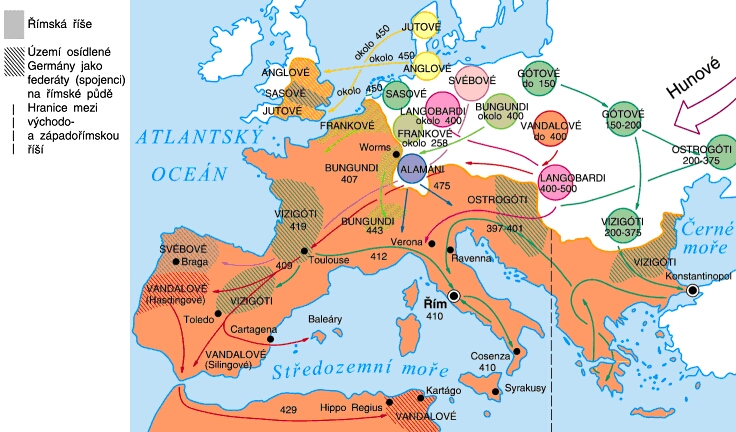
\includegraphics[width=\linewidth]{mapa.jpg}
\end{minipage}

\section*{Pohyby}
\subsection*{Germánské kmeny}
\begin{multicols}{2}
    \begin{description}
        \setlength\itemsep{0.15em}
        \item[Gótové:] S Německo $\rightarrow$ od 2. st. k Černému moři\\
        rozštěpeni na:
        \begin{itemize}
            \item Ostrogóti -- V
            \item Vizigóti -- Z
        \end{itemize}
        \item[Jutové:] Jutský poloostrov
        \item[Anglové, Sasové:] S Německo
        \item[Langobardi:] S Německo západně od Labe
    \end{description}

    \begin{description}
        \setlength\itemsep{0.15em}
        \item[375] Hunové vs. Ostrogóti, Sarmaté\\
            Hunové Ostrogóty ovládli, posunuli na Z $\rightarrow$ narazí na Vizigóty $\rightarrow$ jsou na Balkán
        \item[378] \textsc{bitva u Hadrianopolu}\\
            porážka Římanů, jdou na Apeninský poloostrov
        \item[410] vyplenění Říma, poté dál na JZ Francie
        \item[419 -- 507] Tolosánská říše (u Toulouse)\\
            dále je \uv{vyšťouchnou} Frankové $\Rightarrow$
        \item[(507 -- 711)] Vizigótská říše (dnešní Španělsko)
        \item[(711)] vyvrácení Vizigótské říše Araby
    \end{description}
\end{multicols}

\subsection*{Vandalové}
    mezi Odrou a Vislou $\rightarrow$ do Z Evropy, Pyrenejský pol., přes Gibraltar, v S Africe založili říši -- království Vandalů, v r. \textbf{455} vyplenili Řím, vyvrácení VŘŘ, vůdce Belisar

\subsection*{Hunové}
    na Balkán, poté Z Evropa, \textbf{451} \textsc{bitva u Katalunských polí}, poté se vrací na V

\subsection*{Ostrogóti}
    na S Balkánského pol. v Panonii, ovládli celou Itálii -- král Theodorich (hrobka v Ravenně), Ostrogótské království (493 -- 553), díky VŘŘ a příchodu Langobardů říše zaniká

\subsection*{Langobardi}
    přes naše území do Panonie $\rightarrow$ pak S Itálie, Pavia -- hl. město, říše (568 -- 774), poraženi Karlem Velikým

\subsection*{Frankové}
    Belgie $\rightarrow$ poté Franská říše (galie, 481 -- 843), Karel Veliký

\subsection*{Britské ostrovy}
\begin{minipage}{0.7\textwidth}\raggedleft
    \vspace{-3em}
    \begin{description}
        \setlength\itemsep{0.15em}
        \item[Keltové] S + Z
        \item[Jutové] J Anglie
        \item[Sasové] Temže
        \item[Anglové] SV pobřeží
    \end{description}
    \begin{itemize}
        \setlength\itemsep{0.15em}
        \item[$-$] král Artuš
        \item[$-$] vytváří svá království (Wessex, Sussex, Kent, \dots)
    \end{itemize}
\end{minipage}
\hfill
\noindent\begin{minipage}{0.3\textwidth}
    \vspace{-5em}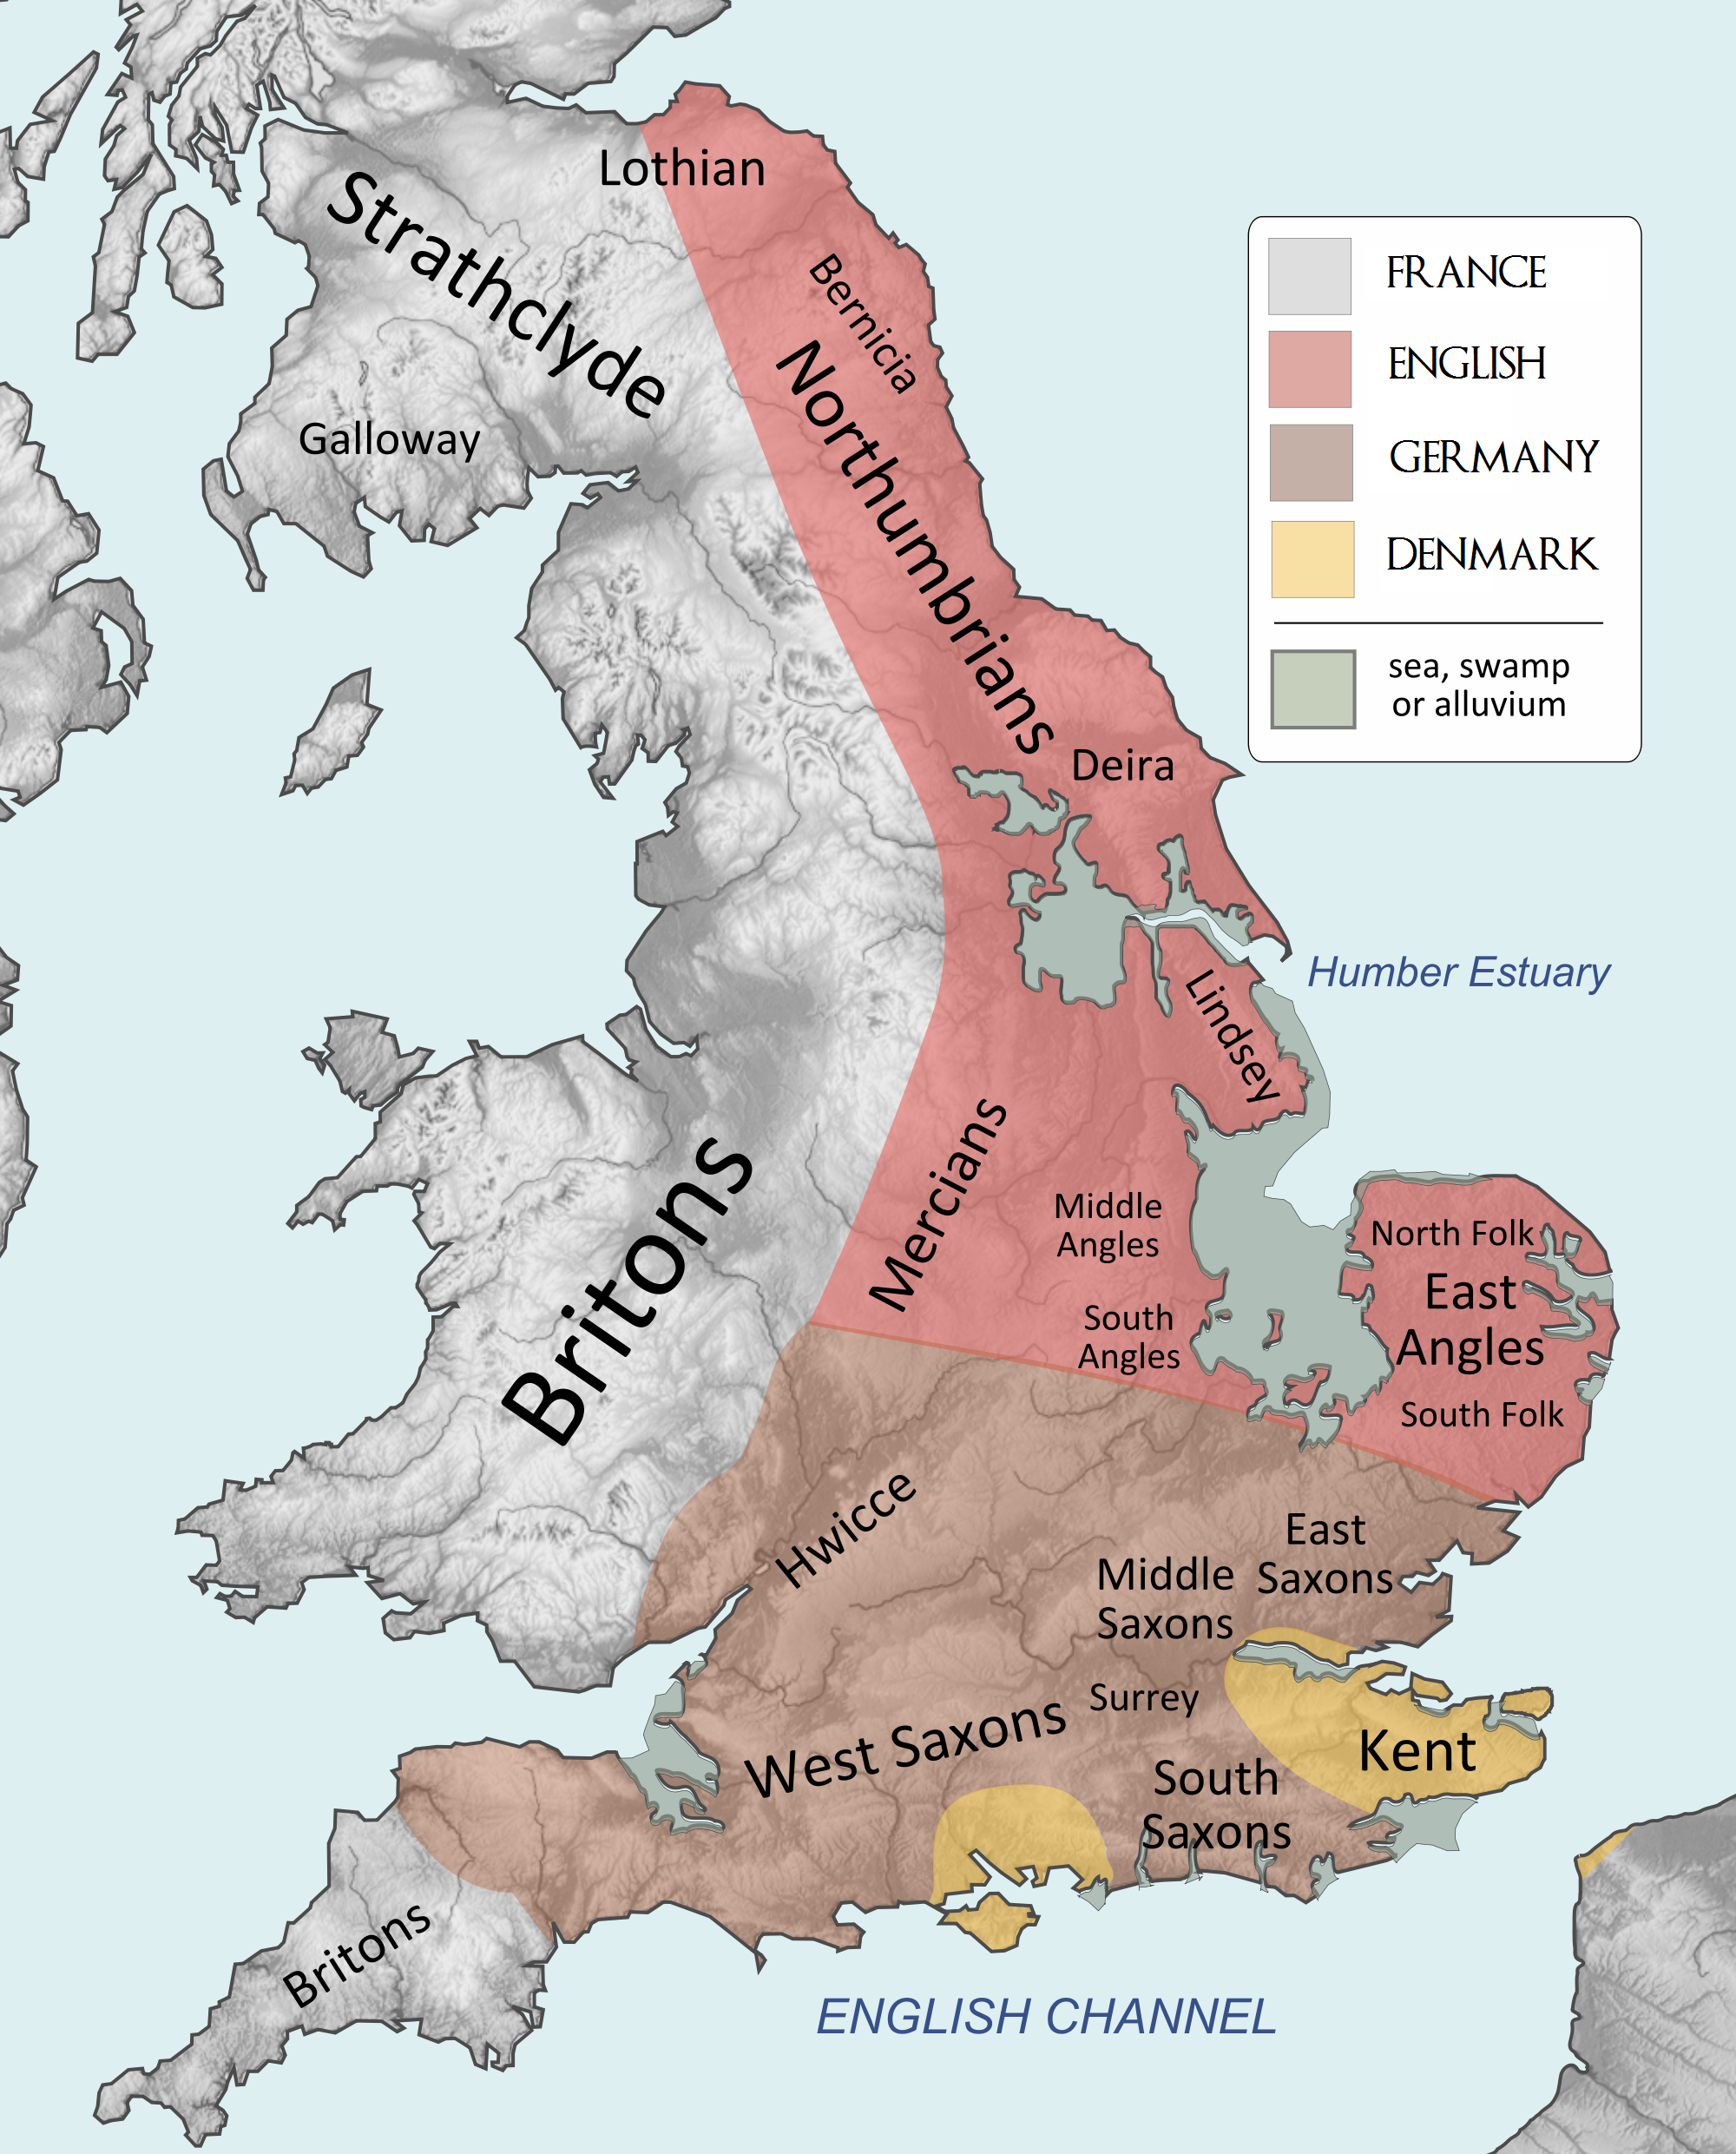
\includegraphics[width=\linewidth]{britanie.png}
\end{minipage}

\vspace{-2em}
\subsection*{Slované}
    původně mezi Vislou a Dněprem, expanze do všech stran:
    \begin{description}
        \setlength\itemsep{0.15em}
        \item[západní:] Češi, Poláci, Slováci, \dots
        \item[východní:] Rusové, Rusíni, \dots
        \item[jižní:] Bilhaři, Srbové, Chorvati, \dots
    \end{description}

\begin{figure}[h]
    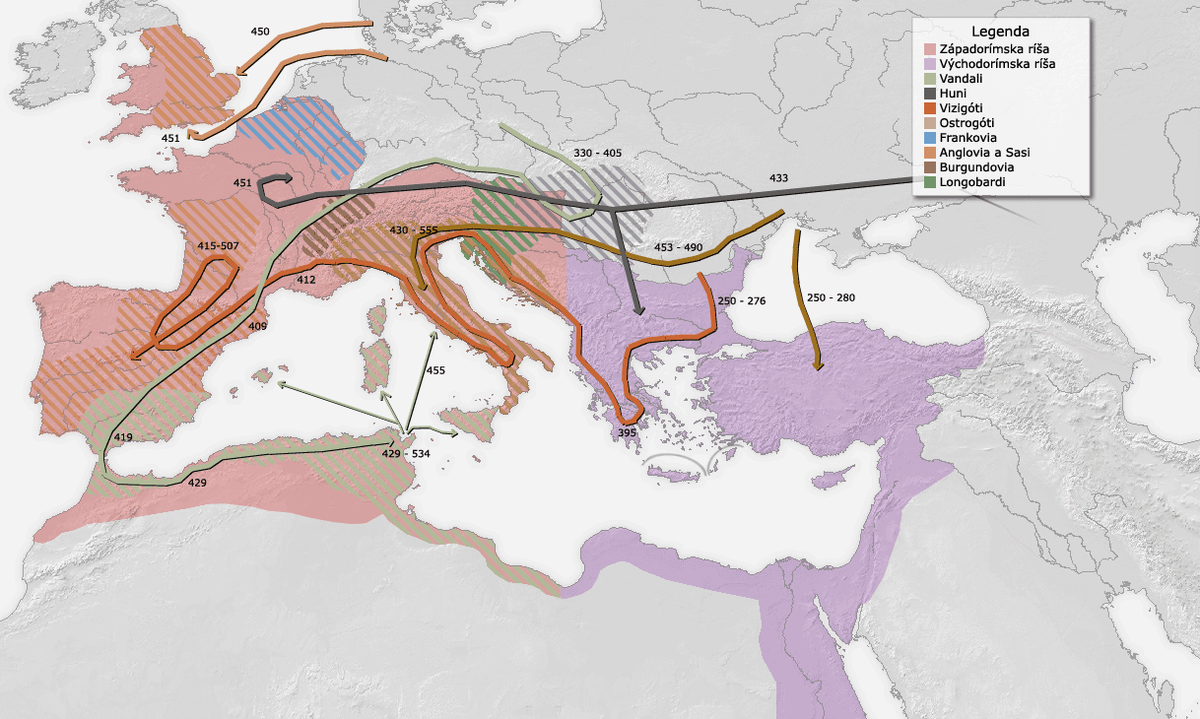
\includegraphics[width=\linewidth]{mapa-celk.png}
\end{figure}

\end{document}
